\chapter{Evaluation}
In this chapter, the results of the research are evaluated against the research objectives set out in Chapter One. Firstly, a plan is proposed, detailing the approach to evaluation the chapter shall follow. The translation models are then evaluated with the existing metrics.
\section{Approach}

\begin{figure}[h]
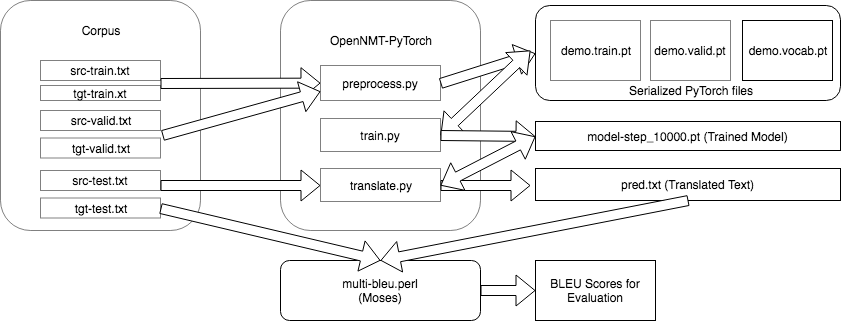
\includegraphics[width=\textwidth]{figures/multibleu.png}
\caption{Evaluation process using BLEU} 
\label{multibleu}
\end{figure}

The training models are initially evaluated using the perplexity parameters available within the OpenNMT toolkit during training and validation. Later the models are evaluated using the BLEU metrics.  

\section{Prediction and Perplexity}
In OpenNMT system, the Prediction scores generated by the system are the cumulative log likelihood of the generated sequence where as the Prediction Average scores are the log likelihood per generated word. Though the Prediction scores are relevant to determine the quality of translation model during the training, but they are not discriminant enough to judge whether the translations are of good quality or bad quality. 

For this research, Perplexity is used as an initial evaluation metric to judge the quality of the translation model. In simpler terms, Perplexity is the measurement of unknown words by the translation model or the words those were not understood by the translation model. Perplexity is considered to be a good indicator to judge the convergence of a model.
As per the formula listed on the Wikipedia page for Perplexity (\citeauthor{wiki:xxx}, \citeyear{wiki:xxx}),
the perplexity of a given model q is defined as,
\begin{equation*}
    b^{-{\frac{1}{N}} \sum_{i=1}^N log_b q(x_i)}
\end{equation*}

,where b is customarily 2. As per \cite{opennmtforum} , in OpenNMT they used $b = e$ (exponential , but could also be b=2) and N is total number of words.
\begin{itemize}
    \item The minimum value of perplexity is when $q(x_i) = 1$ for all $i$ (i.e. predict each sample with the highest confidence), which makes the perplexity equal to $exp(0) = 1.$
    \item The maximum value is when $q(x_i)$ = 0 for all i (i.e. predict each sample with the lowest confidence), which makes the perplexity equal to exp$(+inf) = +inf.$
\end{itemize}
In OpenNMT , there are three types perplexity scores,
\begin{itemize}
   \item \textbf{Training Perplexity} It is the perplexity of the true target data of the training.
    \item \textbf{Validation Perplexity} It is the perplexity of the true target data of the validation.
    \item \textbf{Translation Perplexity} It is the perplexity of the model’s own prediction while creating translations.
\end{itemize}
For this research, the prediction scores and perplexity were evaluated. After the training the models for 100K steps , the model with the lowest validation perplexity was chosen as the baseline model. The models and their corresponding prediction scores and perplexity is showed in Table \ref{bleutable5}.
\section{BLEU}
A method called BLEU (Bilingual Evaluation Understudy) were proposed by \cite{Papineni:2002:BMA:1073083.1073135} for automatic evaluation of machine translation models.According to the authors, \textit{"The closer a machine translation is to a professional
human translation, the better it is"}. The main foundation of the metric is the precision measure. A normal precision score is calculated by dividing the number of word in the candidate text which matches with reference text by the total number of words in the candidate text. But a score which is calculated like that is very unrealistic for machine translation because a poor translation system can over generate reasonable words and score high precision. The authors suggested the use of \textit{modified unigram precision}, in which, firstly the number of times a word appears in the reference sentence is counted, then the total count of each candidate word is clipped to the reference count. Finally the total number clipped counts are divided by the total number un-clipped candidate words. A modified n-gram precision is calculated similarly where the clipped candidate counts are divided by the total number candidate n-grams.BLEU for the test corpus is calculated by taking the geometric mean of the test corpus modified precision scores and then multiplied by an exponential brevity penalty factor. Brevity Penalty Factor and the BLEU score is calculated as follows,

\begin{align*}
    BP &= \begin{cases}
  1 & \text{if } c \ge r\\    
  e^(1-r/c) & \text{if } c\leq r\\    
   \end{cases} 
   \\
BLEU &= BP.exp \Bigg(\sum_{n=1}^N w_n logp_n\Bigg) \\
\end{align*}

The value of BLEU metric ranges from 0 to 1, where a score closer to 1 indicates that the candidate text is more identical to the reference text. \cite{Papineni:2002:BMA:1073083.1073135} research showed that the BLEU scores co-relate very closely with human evaluation and thus it widely considered to be the benchmark for evaluating the machine translation systems. Many researches such as \cite{Callison-Burch06re-evaluatingthe}, \cite{unknown} argued that though BLEU has significant advantages as an evaluation metric for machine translations but an increase in BLEU score doesn't guarantee an improvement in the translation quality. But still,BLEU is widely considered to be the benchmark for machine translations and widely used as an evaluation metric for machine learning tasks (WMT 2017, WAT 2017 etc) in leading conferences. This was the motivation behind using the BLEU metrics for evaluating the translation models in this research. 

For this research, the BLEU scoring tool multi-bleu.perl provided by Moses is used to calculate the BLEU scores for the translated texts. The BLEU scores computed by multi-bleu.perl are multiplied by 100, and it ranges between 0 to 100, with 100 being the candidate text exactly identical to reference text.

\section{Discussion}

The OpenNMT models which were discussed in Section \ref{opennmtmodels} were trained and tested on Nvidia Tesla K80 GPU hosted by the deep learning platform FloydHub \footnote{\url{https://www.floydhub.com/},accessed:15.08.2018}. Nvidia Tesla K80 GPU\footnote{{\url{https://www.nvidia.com/en-us/data-center/tesla-k80/},accessed:20.08.2018}} has specifications of 2x Kepler GK210, Memory size (GDDR5) of 24GB (12GB per GPU), CUDA cores of 4992 ( 2496 per GPU),Memory bandwidth of 480 GB/sec (240 GB/sec per GPU)
and 2.91 Tflops double precision performance with NVIDIA GPU Boost. Table \ref{bleutable4} shows the time taken by the translation models to train for 100K steps on the GPU.

\begin{table}[h!]
\centering
 \begin{tabular}{ |c|c|c| } 
  \hline Model & token/sec & Time (hours)  \\ 
  \hline  OpenNMT-Model-1 &  2077 & 9.3\\
  OpenNMT-Model-2 & 2168 & 11.2\\
  OpenNMT-Model-3 & 1813 & 7.5 \\
  OpenNMT-Model-4 & 2030 & 8.5 \\
  OpenNMT-Model-5 & 1021 & 14.2 \\
  OpenNMT-Model-6 & 1047 & 15.3 \\
  \hline
 \end{tabular}
\caption{Training time of the Translation Models. Each and every model were trained on Nvidia Tesla K80 GPU.}
\label{bleutable4}
\end{table}

In OpenNMT, 100K steps is approximately around 4.5 epochs for the IIT-Bombay Hindi-English Corpus when trained with batch size of 64. The number of epochs for the training process can be calculated by using the following formula,
\begin{equation*}
   \text{ No. of epochs of training} = \frac{\text{No. of steps of training}}{\frac{\text{No. of segments in the Training Corpus}}{\text{Batch Size}}}
\end{equation*}

\cite{DBLP:journals/corr/abs-1709-05820} showed how the BLEU scores of the training models improved with increasing the number of epochs to 20. An ideal experimentation would have been training the models up to 1 million steps as describe by \cite{45610}. But the training was restricted to 100K steps due to limitation of availability of GPU power. 

Table \ref{bleutable5} shows the final Prediction and Perplexity scores of the translation models after the completion of training and validation at the 100K-th step. 
\begin{table}[h!]
\centering
 \begin{tabular}{ |c|c|c|c|c| } 
  \hline Model & \multicolumn{2}{c|}{Training Scores (Step 100K)}  & \multicolumn{2}{c|}{Validation Scores (Step 100K)}\\ 
  \hline & Prediction & Perplexity & Prediction & Perplexity\\
  \hline  OpenNMT-Model-1 & 71.19 & 5.27 & 41.01 &  26.71 \\
  OpenNMT-Model-2 & 79.69 & 3.44&  43.04 & 27.31\\
  OpenNMT-Model-3 & 60.84 & 6.78&  46.36 & 20.96\\
  OpenNMT-Model-4 & 75.78 & 5.62& 47.15  & 21.02\\
  OpenNMT-Model-5 & 76.47 & 5.14& 47.26  & 18.71\\
  OpenNMT-Model-6 & 78.13 & 4.09& 48.54  & 18.54 \\
  \hline
 \end{tabular}
\caption{Prediction and Perplexity of the Translation Models.}
\label{bleutable5}
\end{table}

The validation perplexity of the OpenNMT-Model-6 was 18.54 which was lowest among all, making it a good candidate to be used as the baseline model for the rest of the research. The Fig \ref{multibleu1} shows that the OpenNMT-Model-6 nearly converged during the last phase of validation which indicates a descent translation model.The graph shows how the perplexity is extremely high during the initial phase of the training, and gradually reduces with number of steps. The Fig \ref{multibleu2} shows the prediction scores for during the validation phase of the translation models. OpenNMT models 4 and 6 are having almost same accuracy in the initial phase but with the growing steps OpenNMT-Model-6 outperforms OpenNMT-Model-4 by a descent margin. Both the graphs \ref{multibleu1} and \ref{multibleu2} are generated using  Tensorboard \footnote{{\url{https://www.tensorflow.org/guide/summaries_and_tensorboard},accessed:20.08.2018}}  and smoothed to the value of 0.6. 

\begin{figure}[h]
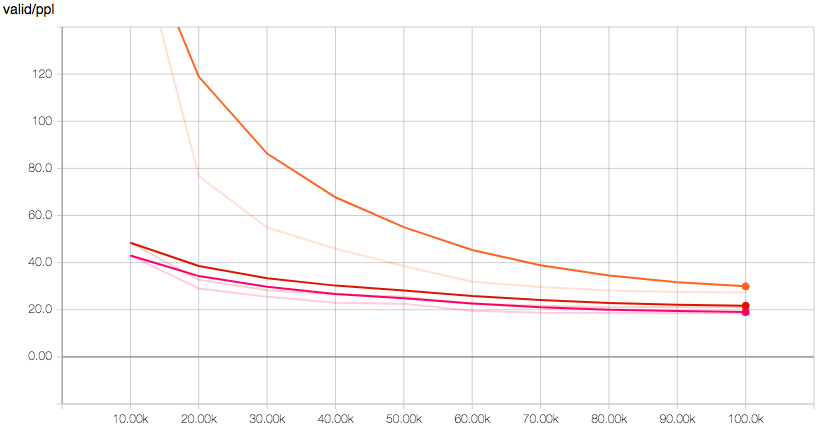
\includegraphics[width=\textwidth]{graphs/graph1.png}
\caption{Graph showing Perplexity for Validation process.Generated using Tensorboard.(ONMT-Model-6 is Pink,ONMT-Model-4 is Red,ONMT-Model-2 is Orange)} 
\label{multibleu2}
\end{figure}

\begin{figure}[h]
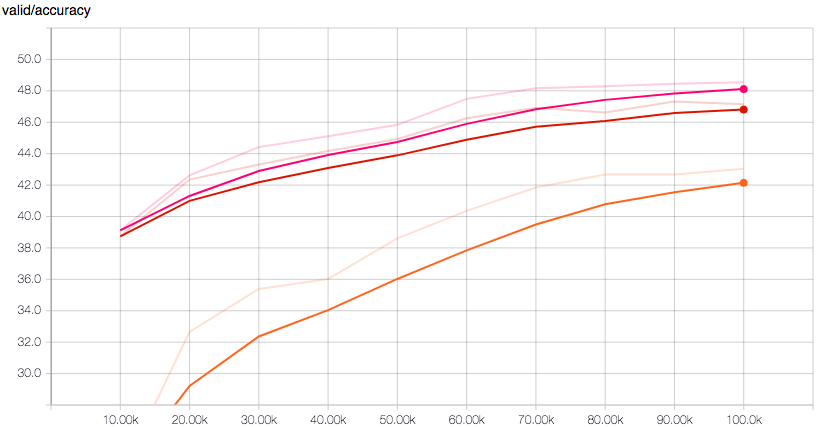
\includegraphics[width=\textwidth]{graphs/graph2.png}
\caption{Graph showing prediction scores for Validation process.Generated using Tensorboard.(ONMT-Model-6 is Pink,ONMT-Model-4 is Red,ONMT-Model-2 is Orange)} 
\label{multibleu1}
\end{figure}

Table \ref{bleutable1} shows the BLEU (Bilingual Evaluation Understudy) scores obtained by the six OpenNMT models against the IIT Bombay Model and Google's NMT. The IIT Bombay Model(\cite{Kunchukuttan2018TheIB}) achieved a BLEU score of 12.23 using the Nematus\footnote{{\url{https://github.com/EdinburghNLP/nematus},accessed:20.08.2018}} baseline model. In WAT 2017\footnote{{\url{http://lotus.kuee.kyoto-u.ac.jp/WAT/WAT2017/},accessed:20.08.2018}} , the convolutional sequence to sequence model by  \cite{Singh2017ComparingRA} achieved a BLEU score 12.23 for English to Hindi translations using the same corpus. In the same workshop, the baseline system designed by \cite{W17-5707} achieved a BLEU score of 13.69. 

Six different models were experimented with to select best baseline model for this research. OpenNMT-Model-6 which was 2- Bi-directional RNNs as Encoder, and 2- LSTM Decoder with an RNN size of 1000 achieved a BLEU score of 14.36 which is way higher than the models described earlier.  Though the Google's NMT has a BLEU score of 32.45, they have a much higher architecture which has 8 layer Encoders and 8 layer decoder which is typically trained simultaneously on 96 K80 GPUs for 1 million steps.The used their private in-production large data sources which seems to be much larger than the publicly available corpora. Whereas , the most successfully trained model in this research used a corpus of 1.5 million sentences and trained for 100K steps on a single K80 GPU. Finally, The OpenNMT-Model-6 is chosen as the baseline model for this research for its lowest perplexity score during validation and highest BLEU score during evaluation.

\begin{table}[h]
\centering
 \begin{tabular}{ |c|c|c| } 
  \hline Model & Architecture & BLEU Score  \\ 
  \hline  IIT Bombay & Nematus- Baseline & 12.23\\
  \hline  IITB-MTG &  RNNS2S(WAT 2017) & 12.23\\
  IITB-MTG & ConvS2S(WAT 2017) & 11.73\\
   XMUNLP-Baseline &  dl4mt tutorial(WAT 2017) & 13.69\\
  \hline  Google & Google NMT & 12.23\\
  \hline  OpenNMT-Model-1 &  4 Layer LSTM Encoder Decoder, SGD & 9.88\\
  OpenNMT-Model-2 & 4 Layer LSTM Encoder Decoder, Adam & 10.09\\
  OpenNMT-Model-3 & 2 Layer LSTM Bi-RNN Encoder Decoder, SGD & 12.89 \\
  OpenNMT-Model-4 & 2 Layer LSTM Bi-RNN Encoder Decoder, Adam & 13.72 \\
  OpenNMT-Model-5 & OpenNMT-Model-3 + RNN Size 1000 & 14.02 \\
  OpenNMT-Model-6 & OpenNMT-Model-4 + RNN Size 1000 & 14.36 \\
  \hline
 \end{tabular}
\caption{BLEU Scores of the Translation Models (English$\rightarrow$Hindi). OpenNMT-Models were the models that were trained for this research.}
\label{bleutable1}
\end{table}

The Back Translation method proposed by \cite{DBLP:journals/corr/SennrichHB15a} was described in Section \ref{backtrans}. Several researches such as \cite{W18-2703} showed how back translation method is effective in case of low language resources but \cite{DBLP:journals/corr/abs-1804-06189}'s research showed how adding too much synthetic data in to the corpus  can deteriorate the BLEU scores.\cite{W17-5707} added 2.5 million synthetic sentences which were created from IIT Bombay Hindi Monolingual Corpus, re-trained their baseline model and improved their BLEU score to 19.79 from 13.69 .For this research , 50,000 synthetic English sentences were used with human generated Hindi sentences from the IIT-Bombay Monolingual Corpus. The decision to use lesser synthetic data was motivated by the fact that, it would have taken more than 24 hours of GPU power to create the synthetic sentences and the training for minimal 100K steps would have taken around 45 hours of GPU training.

Fig \ref{bleutable2} shows the results of the experimentation with the baseline neural translation model. The Back-Translation improved the BLEU score by 0.05 which in-significant, which may be due its less size of 50K compared to 1.5million. The next phase was training domain specific corpus. The Baseline+Back-Translation model was fine-tuned (re-trained) using the TED Talks Hindi-English Corpus. The TED Talks Hindi-English Corpus have around 81K sentences pairs and the model was re-trained for 100K steps which is around 80 epochs. The domain specific training showed an improvement of BLEU score to 14.72.

\begin{table}[h!]
\centering
 \begin{tabular}{ |c|c| } 
  \hline Model & BLEU Score  \\ 
  \hline  XMUNLP(Baseline) &   13.69\\
  XMUNLP(Baseline+Synthetic) &   19.79\\
  \hline  OpenNMT-Model-6 (Baseline) &   14.36\\
  Baseline + Back-Translation & 14.41\\
  Baseline + Back-Trans. + Domain Specific Training & 14.72\\
  \hline
 \end{tabular}
\caption{BLEU Scores of the Translation Models (English$\rightarrow$Hindi)}
\label{bleutable2}
\end{table}

The final phase of the evaluation process was evaluating the models for the domain specific test data. The domain specific test data consisted of 580 English sentences from the Tripoto Blogs. The Baseline English to Hindi model scored 19.48 BLEU on the test data , the back-translations improved the scores slightly to 19.98. The final domain specific translation model obtained a BLEU score of 22.47 which is a significant improvement. These results of the final phase of evaluation addressed the research question posed in the dissertation. For Domain specific translations, domain specific training can improve the BLEU scores by a great margin. 
\begin{table}[h!]
\centering
 \begin{tabular}{ |c|c| } 
  \hline Model & BLEU Score  \\ 
  \hline  OpenNMT-Model-6 (Baseline) &   19.48\\
  Baseline + Back-Translation & 19.98\\
  Baseline + Back-Trans. + Domain Specific Training & 22.47 \\
  \hline
 \end{tabular}
\caption{BLEU Scores of the translation models on domain specific Tripoto test data (English$\rightarrow$Hindi)}
\label{bleutable3}
\end{table}

Figure \ref{translations1} shows the original English sentences and their translations generated by the final translation model. Though the BLEU scores obtained by the translation model is around 22.47, the sentences do reflect good quality of translations. The translation model was able to translate more than 70\% of the words in a given sentences while maintain the grammatical accuracy by changing the word orders when necessary. The translation model failed to translate the nouns and the complicated verb forms which it never encountered during its training phase. There can be two ways to make it better, either by training it with more domain specific data where these nouns are frequent or using a reference transliteration dictionary,which the translation model will look into for unknown words.

\begin{figure}[H]
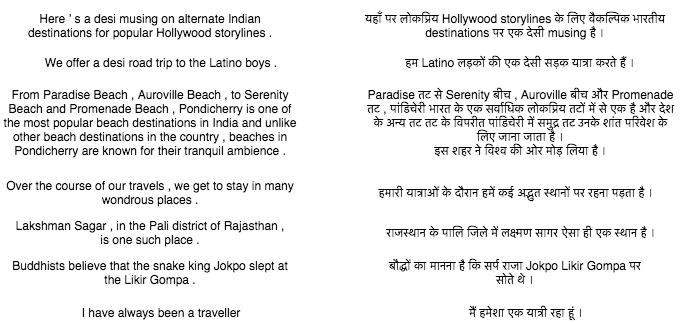
\includegraphics[width=\textwidth]{figures/translations1.png}
\caption{Examples of English$\rightarrow$Hindi translation created by the Baseline+Back-Trans.+Domain Specific Trained Model.The English sentences are excerpts from the domain specific test data which is the actual sentences from the travel blogs.}
\label{translations1}
\end{figure}

\begin{figure}[H]
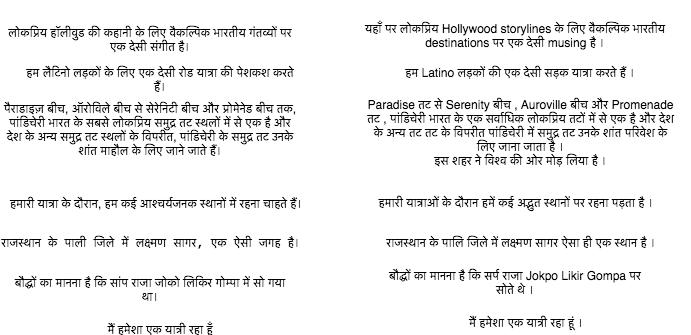
\includegraphics[width=\textwidth]{figures/translation2.png}
\caption{Comparison of English$\rightarrow$Hindi translations. Left side are the translations generated by Google NMT and right side are the translations generated by Baseline+Back-Trans.+Domain Specific Trained Model.} 
\label{translations2}
\end{figure}

Figure \ref{translations2} shows the comparison of the Hindi translations generated by the final model with the Google Translate \footnote{{\url{https://translate.google.com/},accessed:24.08.2018}} which was used as the reference text for evaluation. The comparison shows the most of the sentences generated the translation model used for the research are almost identical to those generated by the Google Translate. The Google Translated sentences have used transliterations for the nouns which don't have any Hindi translations where as the final model uses the original English words. Now talking about the quality of translations, in some of the sentences the final translation model generated more grammatically correct sentences than the Google translate. As Hindi is a more complex language the word orders and word choice plays an important role whole judging the translation quality. Just like English, in Hindi, a same word can have different meanings in different context, so choice of words play an important role to keep the original meaning of the sentence.In some of the sentences, the Google translated sentence changed the whole meaning of the original sentence by using a poor choice of word. The words used by domain specific translation model were much better in terms of language quality, which maintained the original meaning of the sentences.

\section{Summary}
In this part, the evaluation approach was first discussed, which encouraged the choosing of a correct evaluation metric and subsequent evaluation of the research.The first process was the assessment of baseline neural translation model, from the point of view of the primary research question of the dissertation. Several neural translation models were evaluated based on validation perplexity and translation BLEU scores, and the baseline model was selected for further evaluation.

In the Second phase, other implementation such as Back-Translation and Domain Specific Training was taken into consideration, and the performance of the model were evaluated.

The last part of the evaluation considered the evaluation of the previously trained models on the domain specific test data, and and its part in noting the research question posed by the dissertation. The outcomes showed that for domain specific translations , domain specific training can improve the BLEU scores by a significant margin.